\documentclass[xcolor=dvipsnames,10pt]{beamer}
% ********** Style prezentation **********

\usepackage{verbatim}
\usepackage{color}
\usepackage{multimedia}
\usepackage{xmpmulti}
\usepackage[absolute,overlay]{textpos} 
\usepackage{listings}
\usepackage{algorithm}
\usepackage{algorithmic}
\usepackage{amsmath}
\usepackage{pifont}
\usepackage{url}
\usepackage{pict2e}
\usepackage{flushend}
\usepackage{graphicx}
\usepackage{pgf}
\usepackage{url}
\usepackage{tikz}
\usetikzlibrary{calc}
\usetikzlibrary{shapes}
\usetikzlibrary{backgrounds}
\usepackage{pgfplots}
\usepackage{pgfplotstable}

\newcommand{\ignore}[1]{}


\lstset{ %
  language=Java,              
  basicstyle=\footnotesize
}

\mode<presentation>
{
	\usetheme{Warsaw}
}
\definecolor{scarlet}{RGB}{200,0,0}
\setbeamercolor{structure}{fg=scarlet}
\addtobeamertemplate{footline}{
\begin{columns}
  \hfill
\includegraphics[height=.75cm]{unl_clear.pdf}\hspace{.5cm}
\end{columns}
\vspace{2mm}
}{\usebeamercolor[bg]{footline}\hfill\raisebox{1mm}[0mm]{\hspace{2mm}}}

\newcommand\x[1]{\ensuremath{\mathit{#1}}}
\newcommand\lrangle[1]{\ensuremath{\langle#1\rangle}}

\def\ON{\ding{52}}
\def\OF{\ding{55}}
\def~{\phantom{0}}

\setbeamertemplate{navigation symbols}{} %remove if navigation symbols are needed
\setbeamersize{text margin left=5mm, text margin right=5mm} % change margin as you wish

\author{Matt Dwyer}

\title[SE Connections and Directions]{Software Engineering Research}
\subtitle{What's Old is New;Promising Connections and Directions}

\institute{
Department of Computer Science and Engineering\\
University of Nebraska - Lincoln\\
Lincoln, Nebraska USA\\
}

\date{December, 2013}

\begin{document}

\begin{frame}
	\titlepage %displays the title page
\end{frame}

\begin{frame}{Why me?}
Everyone has their own opinion about promising research directions
\vfill
\pause
I'll try to channel a large and diverse group of experts ...
\begin{itemize}
\item collaborators over the past 20 years;
\item PC members I've served with (30+ PCs);
\item ICSE'2014 Future of Software Engineering track participants;
\item the Associate Editors of IEEE Transactions on Software Engineering
\end{itemize}
\pause
\vfill
My bias will show through
\end{frame}

\begin{frame}{Overview}
\tableofcontents %displays the sections of the presentation
\end{frame}

\section{Future of Software Engineering}

\begin{frame}{FoSE Symposium}
Colocated with ICSE every 7 years since 2000 ...
\vfill
\pause

\textcolor{Red}{2000} :
{\footnotesize Testing, 
Requirements, 
Mobility, 
Metrics, 
Analysis, 
Process, 
... on the Internet, 
Mathematical Foundations ..., 
Architecture, 
CM, 
Economics, 
Emprical Studies, 
Reliability, 
Databases in ..., 
Specification, 
Maintenance, 
... for Real-time, 
... for Safety, 
Education, 
Reverse Engineering, 
Performance, 
Security, 
... for Middleware, 
Tools}
\pause

\textcolor{Red}{2007}:
{\footnotesize Testing, 
Requirements, 
Education, 
... and Industry, 
Specification,
... for Automotive, 
... for Mechatronic Systems, 
Analysis, 
Formal Methods, 
Safety, 
Reliability, 
Performance, 
Global, 
... for the Web, 
Collaborative, 
Architecture, 
Middleware, 
Self-managed, 
Deployment, 
Economics, 
Tools, 
Reverse Engineering, 
Search-based ..., 
Empirical Studies}
\pause

\textcolor{Red}{2014}:
{\footnotesize
Testing,
Requirements,
Process,
Mobility,
Maintenance,
Software Product Lines,
... and PL,
... and CAD,
... and Probability,
... and Gaming,
... and Big Data,
... for Healthcare,
... for End-Users,
Traceability,
Social Media,
Certification,
Services,
Large-Scale,
Education
}
\end{frame}

\begin{frame}{FoSE Symposium}
Some topics persist ...
\vfill

\textcolor{Red}{2000} :
{\footnotesize 
\colorbox{Green}{Requirements}, 
Mobility, 
Metrics, 
Analysis, 
\colorbox{Green}{Testing}, 
Process, 
... on the Internet, 
Mathematical Foundations ..., 
Architecture, 
Configuration Management, 
Economics, 
Emprical Studies, 
Reliability, 
Databases in ..., 
Specification, 
Maintenance, 
... for Real-time, 
... for Safety, 
\colorbox{Green}{Education}, 
Reverse Engineering, 
Performance, 
Security, 
... for Middleware, 
Tools}

\textcolor{Red}{2007}:
{\footnotesize 
\colorbox{Green}{Testing}, 
\colorbox{Green}{Requirements}, 
... and Industry, 
Specification,
... for Automotive, 
... for Mechatronic Systems, 
Analysis, 
Formal Methods, 
\colorbox{Green}{Education}, 
Safety, 
Reliability, 
Performance, 
Global, 
... for the Web, 
Collaborative, 
Architecture, 
Middleware, 
Self-managed, 
Deployment, 
Economics, 
Tools, 
Reverse Engineering, 
Search-based ..., 
Empirical Studies
}

\textcolor{Red}{2014}:
{\footnotesize
\colorbox{Green}{Testing},
\colorbox{Green}{Requirements},
Process,
Mobility,
Maintenance,
Software Product Lines,
... and PL,
... and CAD,
... and Probability,
... and Gaming,
... and Big Data,
... for Healthcare,
... for End-Users,
Traceability,
Social Media,
Certification,
Services,
Large-Scale,
\colorbox{Green}{Education}
}
\end{frame}

\begin{frame}{FoSE Symposium}
Some evolve and mature ...
\vfill

\textcolor{Red}{2000} :
{\footnotesize 
Requirements, 
\colorbox{Yellow}{Mobility}, 
Metrics, 
Analysis, 
Testing, 
Process, 
\colorbox{Yellow}{... on the Internet}, 
Mathematical Foundations ..., 
Architecture, 
Configuration Management, 
Economics, 
Emprical Studies, 
Reliability, 
Databases in ..., 
Specification, 
Maintenance, 
... for Real-time, 
... for Safety, 
Education, 
Reverse Engineering, 
Performance, 
Security, 
... for Middleware, 
Tools}

\textcolor{Red}{2007}:
{\footnotesize 
Testing, 
Requirements, 
... and Industry, 
Specification,
... for Automotive, 
... for Mechatronic Systems, 
Analysis, 
Formal Methods, 
Education, 
Safety, 
Reliability, 
Performance, 
Global, 
\colorbox{Yellow}{... for the Web}, 
Collaborative, 
Architecture, 
Middleware, 
Self-managed, 
Deployment, 
Economics, 
Tools, 
Reverse Engineering, 
Search-based ..., 
Empirical Studies
}

\textcolor{Red}{2014}:
{\footnotesize
Testing,
Requirements,
Process,
\colorbox{Yellow}{Mobility},
Maintenance,
Software Product Lines,
... and PL,
... and CAD,
... and Probability,
... and Gaming,
... and Big Data,
... for Healthcare,
... for End-Users,
Traceability,
Social Media,
Certification,
Services,
Large-Scale,
Education
}
\end{frame}

\begin{frame}{FoSE Symposium}
Some evolve and mature ...
\vfill

\textcolor{Red}{2000} :
{\footnotesize 
Requirements, 
Mobility, 
Metrics, 
Analysis, 
Testing, 
Process, 
... on the Internet, 
Mathematical Foundations ..., 
Architecture, 
Configuration Management, 
Economics, 
Emprical Studies, 
Reliability, 
Databases in ..., 
Specification, 
Maintenance, 
... for Real-time, 
\colorbox{Blue}{\textcolor{White}{... for Safety}}, 
Education, 
Reverse Engineering, 
Performance, 
Security, 
... for Middleware, 
Tools}

\textcolor{Red}{2007}:
{\footnotesize 
Testing, 
Requirements, 
... and Industry, 
Specification,
... for Automotive, 
... for Mechatronic Systems, 
Analysis, 
Formal Methods, 
Education, 
\colorbox{Blue}{\textcolor{White}{Safety}}, 
Reliability, 
Performance, 
Global, 
... for the Web, 
Collaborative, 
Architecture, 
Middleware, 
Self-managed, 
Deployment, 
Economics, 
Tools, 
Reverse Engineering, 
Search-based ..., 
Empirical Studies
}

\textcolor{Red}{2014}:
{\footnotesize
Testing,
Requirements,
Process,
Mobility,
Maintenance,
Software Product Lines,
... and PL,
... and CAD,
... and Probability,
... and Gaming,
... and Big Data,
... for Healthcare,
... for End-Users,
Traceability,
Social Media,
\colorbox{Blue}{\textcolor{White}{Certification}},
Services,
Large-Scale,
Education
}
\end{frame}

\begin{frame}{FoSE Symposium}
A noticeable trends towards connections ...
\vfill

\textcolor{Red}{2000} :
{\footnotesize 
Requirements, 
Mobility, 
Metrics, 
Analysis, 
Testing, 
Process, 
... on the Internet, 
Mathematical Foundations ..., 
Architecture, 
Configuration Management, 
Economics, 
Emprical Studies, 
Reliability, 
Databases in ..., 
Specification, 
Maintenance, 
... for Real-time, 
... for Safety, 
Education, 
Reverse Engineering, 
Performance, 
Security, 
... for Middleware, 
Tools}

\textcolor{Red}{2007}:
{\footnotesize 
Testing, 
Requirements, 
\colorbox{Red}{... and Industry}, 
Specification,
\colorbox{Red}{... for Automotive}, 
\colorbox{Red}{... for Mechatronic Systems}, 
Analysis, 
Formal Methods, 
Education, 
Safety, 
Reliability, 
Performance, 
Global, 
... for the Web, 
Collaborative, 
Architecture, 
Middleware, 
Self-managed, 
Deployment, 
Economics, 
Tools, 
Reverse Engineering, 
Search-based ..., 
Empirical Studies
}

\textcolor{Red}{2014}:
{\footnotesize
Testing,
Requirements,
Process,
Mobility,
Maintenance,
Software Product Lines,
\colorbox{Red}{... and PL},
\colorbox{Red}{... and CAD},
\colorbox{Red}{... and Probability},
\colorbox{Red}{... and Gaming},
\colorbox{Red}{... and Big Data},
\colorbox{Red}{... for Healthcare},
\colorbox{Red}{... for End-Users},
Traceability,
Social Media,
Certification,
Services,
Large-Scale,
Education
}
\end{frame}

\section{Repeating history without the doom}

\begin{frame}{Lots of problems from the 1970s remain}
\pause
What's a good test suite?  How can we build them?
\vfill
\pause
How to effectively communicate intended system behavior?
\vfill
\pause
How to spot errors early in development?
\vfill
\pause
How to program with limited resources?
\vfill
\pause
Lots of interesting solutions to these and other problems
\begin{itemize}
\item not fashionable to read old papers
\item ignorance is a missed opportunity
\item devalues progress in the field
\end{itemize}
\end{frame}

\begin{frame}{How can we build good test suites?}
\pause
A test consists of two parts: an input and an expected output
\pause
\vfill
How should we choose inputs?
\begin{itemize}
\item define an equivalence relation on input domain
\item choose a representative from each equivalence class
\end{itemize}
\vfill
\pause
The program tells you what the equivalence relation is
\begin{itemize}
\item one class per executable path
\item {\bf symbolic execution} computes a characteristic function for the class (King 1973)
\end{itemize}
\end{frame}

\begin{frame}{If only it were that easy ...}
\pause
one class per executable path
\begin{itemize}
\item how many paths?
\item when is a path executable?
\end{itemize}
\vfill
\pause
Machines were slow in the 70s and decision procedures were in their infancy.
\vfill
\pause
Rediscovery of symbolic execution and connection with advances in SAT/SMT (Khurshid 2003)
\begin{itemize}
\item 100s of papers in the past decade
\item smart security testing (correctness is lack of vulnerability)
\item Microsoft, Coverity, IBM, Fujitsu, NASA, ...
\end{itemize}
\end{frame}


\begin{frame}{How to spot errors early?}
\pause
The earlier you catch an error the cheaper it is to fix (Boehm 1975 or 1973)
\vfill
\pause
\only<3>{Lots of approaches to pursue this goal}
\only<4->{When do you think people defined a solution for these answers?}
\begin{itemize}
\item What software artifact to check? \onslide<4->{\textcolor{Red}{source code}} 
\item What's an error? \onslide<4->{\textcolor{Red}{user defined flow errors, e.g., no def before use}}
\item How thoroughly do you want to check for errors? \onslide<4->{\textcolor{Red}{all runs}}
\end{itemize}
\vfill
\only<5>{Fosdick 1976}
\end{frame}

\begin{frame}{If only it were that easy ...}
\pause
Analysis needs to be ...
\begin{itemize}
\item fast
\item precise
\end{itemize}
\vfill
\pause
Machines were slow in the 70s and a general theory for such analyses was not available (wait until 1977)
\vfill
\pause
Slow progress over time
\begin{itemize}
\item 100s of papers in the past decade
\item Many companies build tools that do this
\end{itemize}
\end{frame}

\begin{frame}{Lots of new problems since the 1970s}
Development teams are large and distributed
\vfill
\pause
Distributed and parallel execution for performance
\vfill
\pause
Software increasingly used in critical settings
\vfill
\pause
Software increasingly {\em built} by non-software experts
\vfill
\pause
There is a need to leverage ideas from other disciplines
\begin{itemize}
\item study analagous problems outside software engineering
\item master techniques from those disciplines
\item understand how to apply them within software engineering
\end{itemize}
\end{frame}

\section{Connections}

\begin{frame}{Connections: Technologies}
\pause
Big Data
\begin{itemize}
\item e.g., data mining, machine learning, ...
\item software is more than code, e.g., CM, bug repos, discussion forums, execution logs, ...
\item modeling, prediction, estimation, visualization, understanding, ...
\end{itemize}
\vfill
\pause

Natural Language Processing
\begin{itemize}
\item e.g., sentiment analysis, information retrieval, ...
\item software involves natural language, e.g., comments, requirements, licenses, bug reports, ...
\item bridging between natural and formal language artifacts
\end{itemize}
\vfill
\pause

Automated Deduction
\begin{itemize}
\item e.g., model checking, SAT, SMT, ...
\item test generation, verification, code synthesis, optimization, ...
\end{itemize}
\vfill
\pause
Human-oriented SE: HCI, Social Networks, Anthropometry, ...
\end{frame}

\begin{frame}{Connections: Domains}
Everyone needs software, but they aren't SE experts
\begin{itemize}
\item there will be low hanging fruit
\item there will be context that can be exploited
\end{itemize}
\vfill
\pause
Healthcare
\begin{itemize}
\item huge area moving forward
\item significant regulatory and safety issues
\item community built up, e.g., SEHC workshop
\item topics: process modeling, information-flow/privacy for HIPPA, medical devices/CPS, computational medicine, proof generation for FDA aproval
compliance, ...
\end{itemize}
\vfill
\pause
We are working on ...
\begin{itemize}
\item Ecological Modeling, Robotics, and High-Performance Computing
\end{itemize}
\end{frame}

\begin{frame}{Connections: Industry}
\pause
\vfill
Talk to people in local industry
\begin{itemize}
\item what are their pain points?
\item these are likely shared
\end{itemize}
\vfill
People-driven connections take time, but payoff
\begin{itemize}
\item need face-time with practitioners 
\item exchanges: sabbaticals, practitioner-in-residence
\item 1-2 years investment before payoff
\end{itemize}
\pause
\vfill
Examples of big research wins: Healthcare/UMass, Security/KSU
\end{frame}

\begin{frame}{Ask Questions} 
\pause
... they lead in new directions
\vfill
\pause
New questions are great, but so are old questions ...
\begin{itemize}
\item re-ask questions where context has changed
\item re-ask questions where existing answers are inadequate
\end{itemize}
\vfill
\pause
{\large \bf \textcolor{Red}{What makes you confident that your software works correctly?}}
\pause
\begin{itemize}
\item I asked this of some Ecologists I was working with\pause
\item then I asked it of myself
\end{itemize}
\end{frame}

\section{An example from my work}

\begin{frame}{Basic symbolic execution algorithm} 
\begin{algorithm}[H]
\small
\caption{{\tt symbolicExecute}$(l,\phi,m)$}
\begin{algorithmic}
 \WHILE{$\neg branch(l)$}
   \STATE $m \gets m\lrangle{v, e}$
   \STATE $l \gets next(l)$
 \ENDWHILE

 \STATE $c \gets m[\x{cond}(l)]$

 \IF{SAT$(\phi \wedge c)$}
   \STATE {\tt symbolicExecute}$(\x{target}(l), \phi \wedge c, m)$
 \ENDIF

 \IF{SAT$(\phi \wedge \neg c)$}
   \STATE {\tt symbolicExecute}$(\x{next}(l), \phi \wedge \neg c, m)$
 \ENDIF
\end{algorithmic}
\end{algorithm}
\end{frame}

\begin{frame}[fragile]
\frametitle{A simple example ...}
\begin{center}
\begin{lstlisting}
int classify(int a, int b, int c) {
  if (a<=0 || b<=0 || c<=0) return 4;
  int type=0;
  if (a==b) type+=1;
  if (a==c) type+=2;
  if (b==c) type+=3;
  if (type==0) {
    if (a+b<=c || b+c<=a || a+c>=b) type=4;
    else type=1;
    return type;
  }
  if (type>3) type=3;
  else if (type==1 && a+b>c) type=2;
  else if (type==2 && a+c>b) type=2;
  else if (type==3 && b+c>a) type=2;
  else type=4;
  return type;
}
\end{lstlisting}
\end{center}
\end{frame}

\newcommand{\Hilight}{\makebox[0pt][l]{\color{yellow}\rule[-0.45em]{\linewidth}{1.5em}}}
\begin{frame}[fragile]
\frametitle{A simple example ...}
\begin{center}
\begin{lstlisting}[escapechar=\%]
int classify(int a, int b, int c) {
  %\Hilight%if (a<=0 || b<=0 || c<=0) return 4;
  int type=0;
  if (a==b) type+=1;
  if (a==c) type+=2;
  if (b==c) type+=3;
  if (type==0) {
    if (a+b<=c || b+c<=a || a+c>=b) type=4;
    else type=1;
    return type;
  }
  if (type>3) type=3;
  else if (type==1 && a+b>c) type=2;
  else if (type==2 && a+c>b) type=2;
  else if (type==3 && b+c>a) type=2;
  else type=4;
  return type;
}
\end{lstlisting}
\end{center}
\end{frame}

\begin{frame}{Symbolic execution tree}
\begin{center}
\begin{tikzpicture}[scale=0.6]
  \node {\texttt{a$\le$0}}
     child {
       node[xshift=-7mm, yshift=3mm] {\colorbox{Green}{4}}
       edge from parent
     }
     child {
       node[xshift=5mm, yshift=3mm] {$b \le 0$}
       child {
         node[xshift=-7mm, yshift=3mm] {\colorbox{Green}{4}}
         edge from parent
       }
       child {
         node[xshift=5mm, yshift=3mm] {$c \le 0$}
         child {
           node[xshift=-7mm, yshift=3mm] {\colorbox{Green}{4}}
           edge from parent
         }
         child [color=white] {
           node[xshift=5mm, yshift=3mm] {$a=b$}
           child {
             node[xshift=-30mm, yshift=2mm] {$a=c$}
             child {
               node[xshift=-4mm, yshift=3mm] {$b=c$}
               child {
                 node[xshift=0mm, yshift=2mm] {}
                 edge from parent
               }
               child {
                 node[xshift=0mm, yshift=2mm] {}
                 edge from parent
               }
               edge from parent
             }
             child {
               node[xshift=4mm, yshift=3mm] {$b=c$}
               child {
                 node[xshift=-2mm, yshift=2mm] {}
                 edge from parent
               }
               child { 
                 node[xshift=0mm, yshift=2mm] {$a+b>c$}
                 child {
                   node[yshift=2mm] {}
                   edge from parent
                 }
                 child {
                   node[yshift=2mm] {}
                   edge from parent
                 }
                 edge from parent
               }
               edge from parent
             }
             edge from parent
           }
           child {
             node[xshift=10mm, yshift=2mm] {$a=c$}
             child {
               node[xshift=-13mm, yshift=3mm] {$b=c$}
               child {
                 node[xshift=-2mm, yshift=2mm] {}
                 edge from parent
               }
               child {
                 node[xshift=0mm, yshift=2mm] {$a+c>b$}
                 child {
                   node[yshift=2mm] {}
                   edge from parent
                 }
                 child {
                   node[yshift=2mm] {}
                   edge from parent
                 }
                 edge from parent
               }
               edge from parent
             }
             child {
               node[xshift=20mm, yshift=3mm] {$b=c$}
               child {
                 node[xshift=-15mm, yshift=2mm] {$b+c>a$}
                 child {
                   node[yshift=2mm] {}
                   edge from parent
                 }
                 child {
                   node[yshift=2mm] {}
                   edge from parent
                 }
                 edge from parent
               }
               child {
                 node[xshift=0mm, yshift=2mm] {$a+b \le c$}
                 child {
                   node[xshift=-5mm, yshift=2mm] {}
                   edge from parent
                 }
                 child {
                   node[xshift=5mm, yshift=2mm] {$b+c \le a$}
                   child {
                     node[xshift=-5mm, yshift=2mm] {}
                     edge from parent
                   }
                   child {
                     node[xshift=0mm, yshift=2mm] {$a+c \ge b$}
                     child {
                       node[yshift=2mm] {}
                       edge from parent
                     }
                     child {
                       node[yshift=2mm] {}
                       edge from parent
                     }
                     edge from parent
                   }
                   edge from parent
                 }
                 edge from parent
               }
               edge from parent
             }
             edge from parent
           }
           edge from parent
         }
         edge from parent
       }
       edge from parent
     };
\end{tikzpicture}
\end{center}
\end{frame}

\begin{frame}[fragile]
\frametitle{A simple example ...}
\begin{center}
\begin{lstlisting}[escapechar=\%]
int classify(int a, int b, int c) {
  if (a<=0 || b<=0 || c<=0) return 4;
  int type=0;
  %\Hilight%if (a==b) type+=1;
  %\Hilight%if (a==c) type+=2;
  %\Hilight%if (b==c) type+=3;
  if (type==0) {
    if (a+b<=c || b+c<=a || a+c>=b) type=4;
    else type=1;
    return type;
  }
  if (type>3) type=3;
  else if (type==1 && a+b>c) type=2;
  else if (type==2 && a+c>b) type=2;
  else if (type==3 && b+c>a) type=2;
  else type=4;
  return type;
}
\end{lstlisting}
\end{center}
\end{frame}

\begin{frame}{Symbolic execution tree}
\begin{center}
\begin{tikzpicture}[scale=0.6]
  \node {\texttt{a$\le$0}}
     child {
       node[xshift=-7mm, yshift=3mm] {\colorbox{Green}{4}}
       edge from parent
     }
     child {
       node[xshift=5mm, yshift=3mm] {$b \le 0$}
       child {
         node[xshift=-7mm, yshift=3mm] {\colorbox{Green}{4}}
         edge from parent
       }
       child {
         node[xshift=5mm, yshift=3mm] {$c \le 0$}
         child {
           node[xshift=-7mm, yshift=3mm] {\colorbox{Green}{4}}
           edge from parent
         }
         child {
           node[xshift=5mm, yshift=3mm] {$a=b$}
           child {
             node[xshift=-30mm, yshift=2mm] {$a=c$}
             child {
               node[xshift=-4mm, yshift=3mm] {$b=c$}
               child [color=white] {
                 node[xshift=0mm, yshift=2mm] {}
                 edge from parent
               }
               child [color=white] {
                 node[xshift=0mm, yshift=2mm] {}
                 edge from parent
               }
               edge from parent
             }
             child {
               node[xshift=4mm, yshift=3mm] {$b=c$}
               child [color=white] {
                 node[xshift=-2mm, yshift=2mm] {}
                 edge from parent
               }
               child [color=white] { 
                 node[xshift=0mm, yshift=2mm] {$a+b>c$}
                 child {
                   node[yshift=2mm] {}
                   edge from parent
                 }
                 child {
                   node[yshift=2mm] {}
                   edge from parent
                 }
                 edge from parent
               }
               edge from parent
             }
             edge from parent
           }
           child {
             node[xshift=10mm, yshift=2mm] {$a=c$}
             child {
               node[xshift=-13mm, yshift=3mm] {$b=c$}
               child [color=white] {
                 node[xshift=-2mm, yshift=2mm] {}
                 edge from parent
               }
               child [color=white] {
                 node[xshift=0mm, yshift=2mm] {$a+c>b$}
                 child {
                   node[yshift=2mm] {}
                   edge from parent
                 }
                 child {
                   node[yshift=2mm] {}
                   edge from parent
                 }
                 edge from parent
               }
               edge from parent
             }
             child {
               node[xshift=20mm, yshift=3mm] {$b=c$}
               child [color=white] {
                 node[xshift=-15mm, yshift=2mm] {$b+c>a$}
                 child {
                   node[yshift=2mm] {}
                   edge from parent
                 }
                 child {
                   node[yshift=2mm] {}
                   edge from parent
                 }
                 edge from parent
               }
               child [color=white] {
                 node[xshift=0mm, yshift=2mm] {$a+b \le c$}
                 child {
                   node[xshift=-5mm, yshift=2mm] {}
                   edge from parent
                 }
                 child {
                   node[xshift=5mm, yshift=2mm] {$b+c \le a$}
                   child {
                     node[xshift=-5mm, yshift=2mm] {}
                     edge from parent
                   }
                   child {
                     node[xshift=0mm, yshift=2mm] {$a+c \ge b$}
                     child {
                       node[yshift=2mm] {}
                       edge from parent
                     }
                     child {
                       node[yshift=2mm] {}
                       edge from parent
                     }
                     edge from parent
                   }
                   edge from parent
                 }
                 edge from parent
               }
               edge from parent
             }
             edge from parent
           }
           edge from parent
         }
         edge from parent
       }
       edge from parent
     };
\end{tikzpicture}
\end{center}
\end{frame}

\begin{frame}[fragile]
\frametitle{A simple example ...}
\begin{center}
\begin{lstlisting}[escapechar=\%]
int classify(int a, int b, int c) {
  if (a<=0 || b<=0 || c<=0) return 4;
  int type=0;
  if (a==b) type+=1;
  if (a==c) type+=2;
  if (b==c) type+=3;
  if (type==0) {
    if (a+b<=c || b+c<=a || a+c>=b) type=4;
    else type=1;
    return type;
  }
  %\Hilight%if (type>3) type=3;
  %\Hilight%else if (type==1 && a+b>c) type=2;
  %\Hilight%else if (type==2 && a+c>b) type=2;
  %\Hilight%else if (type==3 && b+c>a) type=2;
  %\Hilight%else type=4;
  return type;
}
\end{lstlisting}
\end{center}
\end{frame}

\begin{frame}{Symbolic execution tree}
\begin{center}
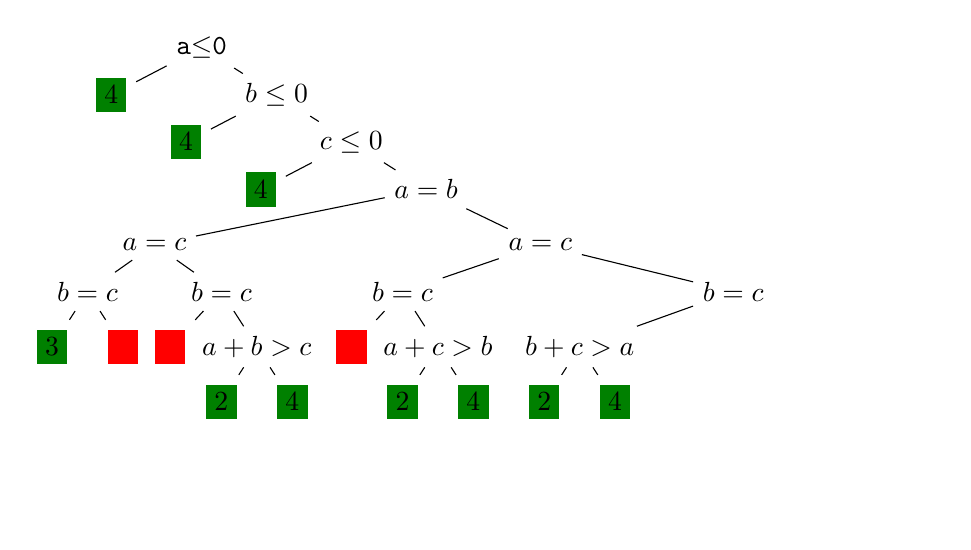
\begin{tikzpicture}[scale=0.6]
  \node {\texttt{a$\le$0}}
     child [color=black] {
       node[xshift=-7mm, yshift=3mm] {\colorbox{Green}{4}}
       edge from parent
     }
     child [color=black] {
       node[xshift=5mm, yshift=3mm] {$b \le 0$}
       child {
         node[xshift=-7mm, yshift=3mm] {\colorbox{Green}{4}}
         edge from parent
       }
       child {
         node[xshift=5mm, yshift=3mm] {$c \le 0$}
         child {
           node[xshift=-7mm, yshift=3mm] {\colorbox{Green}{4}}
           edge from parent
         }
         child {
           node[xshift=5mm, yshift=3mm] {$a=b$}
           child {
             node[xshift=-30mm, yshift=2mm] {$a=c$}
             child {
               node[xshift=-4mm, yshift=3mm] {$b=c$}
               child {
                 node[xshift=0mm, yshift=2mm] {\colorbox{Green}{3}}
                 edge from parent
               }
               child {
                 node[xshift=0mm, yshift=2mm] {\colorbox{Red}{\textcolor{Red}{3}}}
                 edge from parent
               }
               edge from parent
             }
             child {
               node[xshift=4mm, yshift=3mm] {$b=c$}
               child {
                 node[xshift=-2mm, yshift=2mm] {\colorbox{Red}{\textcolor{Red}{3}}}
                 edge from parent
               }
               child { 
                 node[xshift=0mm, yshift=2mm] {$a+b>c$}
                 child {
                   node[yshift=2mm] {\colorbox{Green}{2}}
                   edge from parent
                 }
                 child {
                   node[yshift=2mm] {\colorbox{Green}{4}}
                   edge from parent
                 }
                 edge from parent
               }
               edge from parent
             }
             edge from parent
           }
           child {
             node[xshift=10mm, yshift=2mm] {$a=c$}
             child {
               node[xshift=-13mm, yshift=3mm] {$b=c$}
               child {
                 node[xshift=-2mm, yshift=2mm] {\colorbox{Red}{\textcolor{Red}{3}}}
                 edge from parent
               }
               child {
                 node[xshift=0mm, yshift=2mm] {$a+c>b$}
                 child {
                   node[yshift=2mm] {\colorbox{Green}{2}}
                   edge from parent
                 }
                 child {
                   node[yshift=2mm] {\colorbox{Green}{4}}
                   edge from parent
                 }
                 edge from parent
               }
               edge from parent
             }
             child {
               node[xshift=20mm, yshift=3mm] {$b=c$}
               child {
                 node[xshift=-15mm, yshift=2mm] {$b+c>a$}
                 child {
                   node[yshift=2mm] {\colorbox{Green}{2}}
                   edge from parent
                 }
                 child {
                   node[yshift=2mm] {\colorbox{Green}{4}}
                   edge from parent
                 }
                 edge from parent
               }
               child [color=white] {
                 node[xshift=0mm, yshift=2mm] {$a+b \le c$}
                 child {
                   node[xshift=-5mm, yshift=2mm] {}
                   edge from parent
                 }
                 child {
                   node[xshift=5mm, yshift=2mm] {$b+c \le a$}
                   child {
                     node[xshift=-5mm, yshift=2mm] {}
                     edge from parent
                   }
                   child {
                     node[xshift=0mm, yshift=2mm] {$a+c \ge b$}
                     child {
                       node[yshift=2mm] {}
                       edge from parent
                     }
                     child {
                       node[yshift=2mm] {}
                       edge from parent
                     }
                     edge from parent
                   }
                   edge from parent
                 }
                 edge from parent
               }
               edge from parent
             }
             edge from parent
           }
           edge from parent
         }
         edge from parent
       }
       edge from parent
     };
\end{tikzpicture}
\end{center}
\end{frame}

\begin{frame}[fragile]
\frametitle{A simple example ...}
\begin{center}
\begin{lstlisting}[escapechar=\%]
int classify(int a, int b, int c) {
  if (a<=0 || b<=0 || c<=0) return 4;
  int type=0;
  if (a==b) type+=1;
  if (a==c) type+=2;
  if (b==c) type+=3;
  if (type==0) {
    %\Hilight%if (a+b<=c || b+c<=a || a+c>=b) type=4;
    %\Hilight%else type=1;
    %\Hilight%return type;
  }
  if (type>3) type=3;
  else if (type==1 && a+b>c) type=2;
  else if (type==2 && a+c>b) type=2;
  else if (type==3 && b+c>a) type=2;
  else type=4;
  return type;
}
\end{lstlisting}
\end{center}
\end{frame}

\begin{frame}{Symbolic execution tree}
\begin{center}
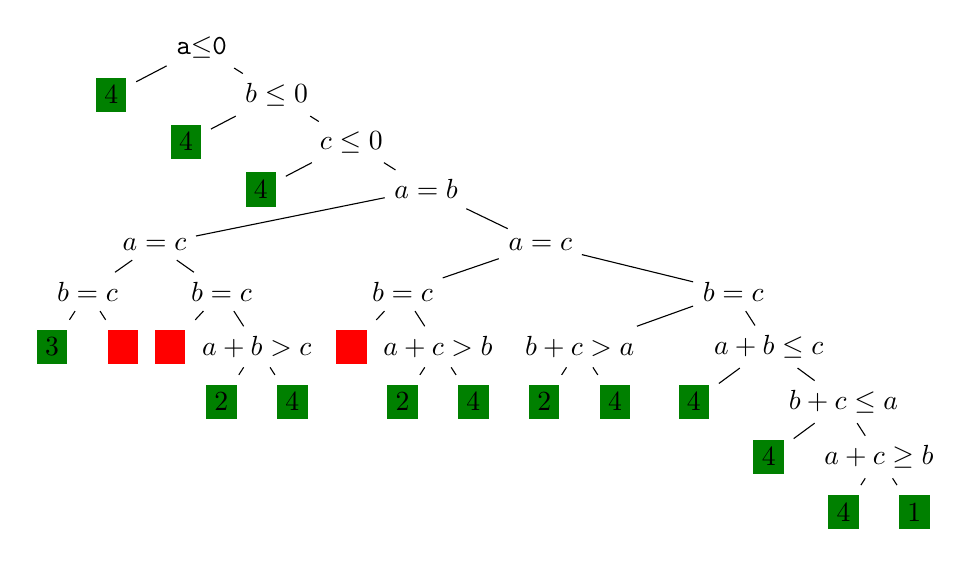
\begin{tikzpicture}[scale=0.6]
  \node {\texttt{a$\le$0}}
     child [color=black] {
       node[xshift=-7mm, yshift=3mm] {\colorbox{Green}{4}}
       edge from parent
     }
     child [color=black] {
       node[xshift=5mm, yshift=3mm] {$b \le 0$}
       child {
         node[xshift=-7mm, yshift=3mm] {\colorbox{Green}{4}}
         edge from parent
       }
       child {
         node[xshift=5mm, yshift=3mm] {$c \le 0$}
         child {
           node[xshift=-7mm, yshift=3mm] {\colorbox{Green}{4}}
           edge from parent
         }
         child {
           node[xshift=5mm, yshift=3mm] {$a=b$}
           child {
             node[xshift=-30mm, yshift=2mm] {$a=c$}
             child {
               node[xshift=-4mm, yshift=3mm] {$b=c$}
               child {
                 node[xshift=0mm, yshift=2mm] {\colorbox{Green}{3}}
                 edge from parent
               }
               child {
                 node[xshift=0mm, yshift=2mm] {\colorbox{Red}{\textcolor{Red}{3}}}
                 edge from parent
               }
               edge from parent
             }
             child {
               node[xshift=4mm, yshift=3mm] {$b=c$}
               child {
                 node[xshift=-2mm, yshift=2mm] {\colorbox{Red}{\textcolor{Red}{3}}}
                 edge from parent
               }
               child { 
                 node[xshift=0mm, yshift=2mm] {$a+b>c$}
                 child {
                   node[yshift=2mm] {\colorbox{Green}{2}}
                   edge from parent
                 }
                 child {
                   node[yshift=2mm] {\colorbox{Green}{4}}
                   edge from parent
                 }
                 edge from parent
               }
               edge from parent
             }
             edge from parent
           }
           child {
             node[xshift=10mm, yshift=2mm] {$a=c$}
             child {
               node[xshift=-13mm, yshift=3mm] {$b=c$}
               child {
                 node[xshift=-2mm, yshift=2mm] {\colorbox{Red}{\textcolor{Red}{3}}}
                 edge from parent
               }
               child {
                 node[xshift=0mm, yshift=2mm] {$a+c>b$}
                 child {
                   node[yshift=2mm] {\colorbox{Green}{2}}
                   edge from parent
                 }
                 child {
                   node[yshift=2mm] {\colorbox{Green}{4}}
                   edge from parent
                 }
                 edge from parent
               }
               edge from parent
             }
             child {
               node[xshift=20mm, yshift=3mm] {$b=c$}
               child {
                 node[xshift=-15mm, yshift=2mm] {$b+c>a$}
                 child {
                   node[yshift=2mm] {\colorbox{Green}{2}}
                   edge from parent
                 }
                 child {
                   node[yshift=2mm] {\colorbox{Green}{4}}
                   edge from parent
                 }
                 edge from parent
               }
               child {
                 node[xshift=0mm, yshift=2mm] {$a+b \le c$}
                 child {
                   node[xshift=-5mm, yshift=2mm] {\colorbox{Green}{4}}
                   edge from parent
                 }
                 child {
                   node[xshift=5mm, yshift=2mm] {$b+c \le a$}
                   child {
                     node[xshift=-5mm, yshift=2mm] {\colorbox{Green}{4}}
                     edge from parent
                   }
                   child {
                     node[xshift=0mm, yshift=2mm] {$a+c \ge b$}
                     child {
                       node[yshift=2mm] {\colorbox{Green}{4}}
                       edge from parent
                     }
                     child {
                       node[yshift=2mm] {\colorbox{Green}{1}}
                       edge from parent
                     }
                     edge from parent
                   }
                   edge from parent
                 }
                 edge from parent
               }
               edge from parent
             }
             edge from parent
           }
           edge from parent
         }
         edge from parent
       }
       edge from parent
     };
\end{tikzpicture}
\end{center}
\end{frame}

\begin{frame}{Some observations}
\begin{itemize}
\item There are 14 distinct paths (Green): from 1 to 9 branches
\item 1 path returns ``scalene'' (1); 3 return ``isoscelese'' (2); and 1 returns ``equilateral'' (3)
\item 3 paths are pruned because constraints are unsat (Red)
\item Interesting symmetries are involved in the ``isoscelese'' and unsat cases
\end{itemize}
\end{frame}

\begin{frame}{Analyzing program behavior}
The symbolic execution could be used to ...
\begin{itemize}
\item check contracts, e.g., if $a=b=c$ then $return=3$
\item generate a suite of 14 thorough tests
\item demonstrate that it is possible to return values $[1,4]$
\end{itemize}
... and support answering other yes/no questions about program behavior.
\end{frame}

\begin{frame}{Moving beyond yes/no questions}
We were interested in exploring how to ...
\begin{itemize}
\item determine the chance that a contract holds (1 is a special case)
\item focus testing on {\em rare} paths (likely ones are easy to hit)
\item determine how frequently a given value is returned
\end{itemize}
... to quantify confidence in program behavior.
\end{frame}

\begin{frame}{Assume \texttt{int}s are drawn uniformly from $[-1000,1000]$}
\begin{center}
\pgfdeclarelayer{foreground}
\pgfsetlayers{main,foreground}
\begin{tikzpicture}[scale=0.6]
  \node {\texttt{a$\le$0}}
     child [color=black] {
       node[xshift=-7mm, yshift=3mm] {\colorbox{Green}{4}}
       edge from parent
     }
     child [color=black] {
       node[xshift=5mm, yshift=3mm] {$b \le 0$}
       child {
         node[xshift=-7mm, yshift=3mm] {\colorbox{Green}{4}}
         edge from parent
       }
       child {
         node[xshift=5mm, yshift=3mm] {$c \le 0$}
         child {
           node[xshift=-7mm, yshift=3mm] {\colorbox{Green}{4}}
           edge from parent
         }
         child {
           node[name=reference, xshift=5mm, yshift=3mm] {$a=b$}
           child {
             node[xshift=-30mm, yshift=2mm] {$a=c$}
             child {
               node[xshift=-4mm, yshift=3mm] {$b=c$}
               child {
                 node[xshift=0mm, yshift=2mm] {\colorbox{Green}{3}}
                 edge from parent
               }
               child {
                 node[xshift=0mm, yshift=2mm] {\colorbox{Red}{\textcolor{Red}{3}}}
                 edge from parent
               }
               edge from parent
             }
             child {
               node[xshift=4mm, yshift=3mm] {$b=c$}
               child {
                 node[xshift=-2mm, yshift=2mm] {\colorbox{Red}{\textcolor{Red}{3}}}
                 edge from parent
               }
               child { 
                 node[xshift=0mm, yshift=2mm] {$a+b>c$}
                 child {
                   node[yshift=2mm] {\colorbox{Green}{2}}
                   edge from parent
                 }
                 child {
                   node[yshift=2mm] {\colorbox{Green}{4}}
                   edge from parent
                 }
                 edge from parent
               }
               edge from parent
             }
             edge from parent
           }
           child {
             node[xshift=10mm, yshift=2mm] {$a=c$}
             child {
               node[xshift=-13mm, yshift=3mm] {$b=c$}
               child {
                 node[xshift=-2mm, yshift=2mm] {\colorbox{Red}{\textcolor{Red}{3}}}
                 edge from parent
               }
               child {
                 node[xshift=0mm, yshift=2mm] {$a+c>b$}
                 child {
                   node[yshift=2mm] {\colorbox{Green}{2}}
                   edge from parent
                 }
                 child {
                   node[yshift=2mm] {\colorbox{Green}{4}}
                   edge from parent
                 }
                 edge from parent
               }
               edge from parent
             }
             child {
               node[xshift=20mm, yshift=3mm] {$b=c$}
               child {
                 node[xshift=-15mm, yshift=2mm] {$b+c>a$}
                 child {
                   node[yshift=2mm] {\colorbox{Green}{2}}
                   edge from parent
                 }
                 child {
                   node[yshift=2mm] {\colorbox{Green}{4}}
                   edge from parent
                 }
                 edge from parent
               }
               child {
                 node[xshift=0mm, yshift=2mm] {$a+b \le c$}
                 child {
                   node[xshift=-5mm, yshift=2mm] {\colorbox{Green}{4}}
                   edge from parent
                 }
                 child {
                   node[xshift=5mm, yshift=2mm] {$b+c \le a$}
                   child {
                     node[xshift=-5mm, yshift=2mm] {\colorbox{Green}{4}}
                     edge from parent
                   }
                   child {
                     node[xshift=0mm, yshift=2mm] {$a+c \ge b$}
                     child {
                       node[yshift=2mm] {\colorbox{Green}{4}}
                       edge from parent
                     }
                     child {
                       node[yshift=2mm] {\colorbox{Green}{1}}
                       edge from parent
                     }
                     edge from parent
                   }
                   edge from parent
                 }
                 edge from parent
               }
               edge from parent
             }
             edge from parent
           }
           edge from parent
         }
         edge from parent
       }
       edge from parent
     };

   \begin{pgfonlayer}{foreground}
      \node[name=first, xshift=30mm, yshift=6mm, above of=reference] 
         {\large Likelihood that \texttt{classify} returns equilateral?}; 
   \end{pgfonlayer}

\end{tikzpicture}
\end{center}
\end{frame}

\begin{frame}{Assume \texttt{int}s are drawn uniformly from $[-1000,1000]$}
\begin{center}
\pgfdeclarelayer{foreground}
\pgfsetlayers{main,foreground}
\begin{tikzpicture}[scale=0.6]
  \node {\texttt{a$\le$0}}
     child [color=white] {
       node[xshift=-7mm, yshift=3mm] {}
       edge from parent
     }
     child {
       node[xshift=5mm, yshift=3mm] {$b \le 0$}
       child [color=white] {
         node[xshift=-7mm, yshift=3mm] {}
         edge from parent
       }
       child {
         node[xshift=5mm, yshift=3mm] {$c \le 0$}
         child [color=white] {
           node[xshift=-7mm, yshift=3mm] {}
           edge from parent
         }
         child {
           node[name=reference, xshift=5mm, yshift=3mm] {$a=b$}
           child {
             node[xshift=-30mm, yshift=2mm] {$a=c$}
             child {
               node[xshift=-4mm, yshift=3mm] {$b=c$}
               child {
                 node[name=ref2, xshift=0mm, yshift=2mm] {\colorbox{Green}{3}}
                 edge from parent
               }
               child [color=white]{
                 node[xshift=0mm, yshift=2mm] {}
                 edge from parent
               }
               edge from parent
             }
             child [color=white] {
               node[xshift=4mm, yshift=3mm] {$b=c$}
               child {
                 node[xshift=-2mm, yshift=2mm] {}
                 edge from parent
               }
               child { 
                 node[xshift=0mm, yshift=2mm] {$a+b>c$}
                 child {
                   node[yshift=2mm] {}
                   edge from parent
                 }
                 child {
                   node[yshift=2mm] {}
                   edge from parent
                 }
                 edge from parent
               }
               edge from parent
             }
             edge from parent
           }
           child [color=white] {
             node[xshift=10mm, yshift=2mm] {$a=c$}
             child [color=white] {
               node[xshift=-13mm, yshift=3mm] {$b=c$}
               child {
                 node[xshift=-2mm, yshift=2mm] {}
                 edge from parent
               }
               child {
                 node[xshift=0mm, yshift=2mm] {$a+c>b$}
                 child {
                   node[yshift=2mm] {}
                   edge from parent
                 }
                 child {
                   node[yshift=2mm] {}
                   edge from parent
                 }
                 edge from parent
               }
               edge from parent
             }
             child {
               node[xshift=20mm, yshift=3mm] {$b=c$}
               child [color=white] {
                 node[xshift=-15mm, yshift=2mm] {$b+c>a$}
                 child {
                   node[yshift=2mm] {}
                   edge from parent
                 }
                 child {
                   node[yshift=2mm] {}
                   edge from parent
                 }
                 edge from parent
               }
               child {
                 node[xshift=0mm, yshift=2mm] {$a+b \le c$}
                 child {
                   node[xshift=-5mm, yshift=2mm] {}
                   edge from parent
                 }
                 child {
                   node[xshift=5mm, yshift=2mm] {$b+c \le a$}
                   child {
                     node[xshift=-5mm, yshift=2mm] {}
                     edge from parent
                   }
                   child {
                     node[xshift=0mm, yshift=2mm] {$a+c \ge b$}
                     child {
                       node[yshift=2mm] {}
                       edge from parent
                     }
                     child {
                       node[yshift=2mm] {}
                       edge from parent
                     }
                     edge from parent
                   }
                   edge from parent
                 }
                 edge from parent
               }
               edge from parent
             }
             edge from parent
           }
           edge from parent
         }
         edge from parent
       }
       edge from parent
     };

   \begin{pgfonlayer}{foreground}
      \node[name=first, xshift=30mm, yshift=6mm, above of=reference] 
         {\large Likelihood that \texttt{classify} returns equilateral?}; 
       \pause
       \node[name=pc, right of=ref2, xshift=40mm] 
          {$\neg(a\le0) \wedge \neg(b\le0) \wedge \neg(c\le0) \wedge (a=b) \wedge (a=c) \wedge (b=c)$}; 
       \pause
       \node[name=question, below of=pc] 
          {How many inputs satisfy this path condition?};
       \pause
       \node[name=answer, below of=question] 
          {1000};
       \pause
       \node[name=firstanswer, below of=first] 
          {$1.25e^{-7}$};
   \end{pgfonlayer}

\end{tikzpicture}
\end{center}
\end{frame}

\ignore{
\begin{frame}{Assume \texttt{int}s are drawn uniformly from $[-1000,1000]$}
\begin{center}
\pgfdeclarelayer{foreground}
\pgfsetlayers{main,foreground}
\begin{tikzpicture}[scale=0.6]
  \node {\texttt{a$\le$0}}
     child [color=white] {
       node[xshift=-7mm, yshift=3mm] {}
       edge from parent
     }
     child [color=black] {
       node[xshift=5mm, yshift=3mm] {$b \le 0$}
       child [color=white] {
         node[xshift=-7mm, yshift=3mm] {}
         edge from parent
       }
       child {
         node[xshift=5mm, yshift=3mm] {$c \le 0$}
         child [color=white] {
           node[xshift=-7mm, yshift=3mm] {}
           edge from parent
         }
         child {
           node[name=reference, xshift=5mm, yshift=3mm] {$a=b$}
           child {
             node[xshift=-30mm, yshift=2mm] {$a=c$}
             child [color=white] {
               node[xshift=-4mm, yshift=3mm] {$b=c$}
               child {
                 node[xshift=0mm, yshift=2mm] {}
                 edge from parent
               }
               child {
                 node[xshift=0mm, yshift=2mm] {}
                 edge from parent
               }
               edge from parent
             }
             child {
               node[xshift=4mm, yshift=3mm] {$b=c$}
               child [color=white] {
                 node[xshift=-2mm, yshift=2mm] {}
                 edge from parent
               }
               child { 
                 node[xshift=0mm, yshift=2mm] {$a+b>c$}
                 child {
                   node[yshift=2mm] {\colorbox{Green}{2}}
                   edge from parent
                 }
                 child [color=white] {
                   node[yshift=2mm] {}
                   edge from parent
                 }
                 edge from parent
               }
               edge from parent
             }
             edge from parent
           }
           child {
             node[xshift=10mm, yshift=2mm] {$a=c$}
             child {
               node[xshift=-13mm, yshift=3mm] {$b=c$}
               child [color=white] {
                 node[xshift=-2mm, yshift=2mm] {}
                 edge from parent
               }
               child {
                 node[xshift=0mm, yshift=2mm] {$a+c>b$}
                 child {
                   node[yshift=2mm] {\colorbox{Green}{2}}
                   edge from parent
                 }
                 child [color=white] {
                   node[yshift=2mm] {}
                   edge from parent
                 }
                 edge from parent
               }
               edge from parent
             }
             child {
               node[xshift=20mm, yshift=3mm] {$b=c$}
               child {
                 node[xshift=-15mm, yshift=2mm] {$b+c>a$}
                 child {
                   node[yshift=2mm] {\colorbox{Green}{2}}
                   edge from parent
                 }
                 child [color=white] {
                   node[yshift=2mm] {}
                   edge from parent
                 }
                 edge from parent
               }
               child [color=white] {
                 node[xshift=0mm, yshift=2mm] {$a+b \le c$}
                 child {
                   node[xshift=-5mm, yshift=2mm] {}
                   edge from parent
                 }
                 child {
                   node[xshift=5mm, yshift=2mm] {$b+c \le a$}
                   child {
                     node[xshift=-5mm, yshift=2mm] {}
                     edge from parent
                   }
                   child {
                     node[xshift=0mm, yshift=2mm] {$a+c \ge b$}
                     child {
                       node[yshift=2mm] {}
                       edge from parent
                     }
                     child {
                       node[yshift=2mm] {}
                       edge from parent
                     }
                     edge from parent
                   }
                   edge from parent
                 }
                 edge from parent
               }
               edge from parent
             }
             edge from parent
           }
           edge from parent
         }
         edge from parent
       }
       edge from parent
     };

   \begin{pgfonlayer}{foreground}
      \node[name=first, xshift=30mm, yshift=6mm, above of=reference] 
         {\large Likelihood that \texttt{classify} returns isosceles?}; \pause
      \node[name=first, below of=first] 
         {$2.80e^{-4}$}; 
   \end{pgfonlayer}

\end{tikzpicture}
\end{center}
\end{frame}
}

\begin{frame}{Some observations}
\begin{itemize}
\item You may be able to calculate these probabilities because you know about triangles.
\item We want to calculate the probability that the program executes a certain way ...
\begin{itemize}
\item returns a value, reaches a statement, ...
\end{itemize}
\item Adapting symbolic execution to perform these computations involves ...
\begin{itemize}
\item calculating the paths of interest
\item calculating the probability of taking those paths
\item combining those probabilities appropriately
\end{itemize}
\end{itemize}
\end{frame}

\begin{frame}{Probabilistic symbolic execution algorithm} 
\begin{algorithm}[H]
\small
\caption{{\tt probSymbolicExecute}$(l,\phi,m,\colorbox{yellow}{p})$}
\begin{algorithmic}
 \WHILE{$\neg branch(l)$}
   \STATE $m \gets m\lrangle{v, e}$
   \STATE $l \gets next(l)$
 \ENDWHILE

 \STATE $c \gets m[\x{cond}(l)]$

%pr(b | p) = pr(b & p) / pr(p)
%pr(b | m) = pr(b & m) / pr(m)

 \STATE \colorbox{yellow}{$\phi' \gets \x{slice}(\phi, c)$}
 \STATE \colorbox{yellow}{$p_c \gets \x{prob}(\phi' \land c) /\x{prob}(\phi')$}

 \IF{SAT$(\phi' \wedge c)$}
   \STATE {\tt probSymbolicExecute}$(target(l), \phi \wedge c, m,$\colorbox{yellow}{$p*p_c$}$)$
 \ENDIF

 \IF{SAT$(\phi' \wedge \neg c)$}
   \STATE {\tt probSymbolicExecute}$(next(l), \phi \wedge \neg c, m,$\colorbox{yellow}{$p*(1-p_c)$}$)$
 \ENDIF
\end{algorithmic}
\end{algorithm}
\end{frame}

\begin{frame}{Key algorithmic features}
Slicing the path condition, i.e., $\x{slice}(\phi,c)$
\begin{itemize}
\item reduces formula size which reduces cost of $\x{prob}(\cdot)$
\item exposes opportunities for reusing computation in $\x{prob}(\cdot)$
\end{itemize}
\pause
Calculating the conditional probability $p_c$ of $c$
\begin{itemize}
\item allows inference of off-branch probability, i.e., $p*(1-p_c)$
\item depth-first nature of symbolic execution ensures that $prob(\phi')$ will be reused
\item slicing does not affect calculation of $p_c$ ($\phi-\phi'$ factored out)
\end{itemize}
\pause
This allows the algorithm to compute path probabilities cost-effectively.
\end{frame}


%% in the following include the probabilities
%%   - Cyan ones are inferred (negated branch)
%%   - Orange ones are computed from reused prob(.) calls

\begin{frame}{Probabilistic symbolic execution tree}
\begin{center}
\pgfdeclarelayer{foreground}
\pgfsetlayers{main,foreground}
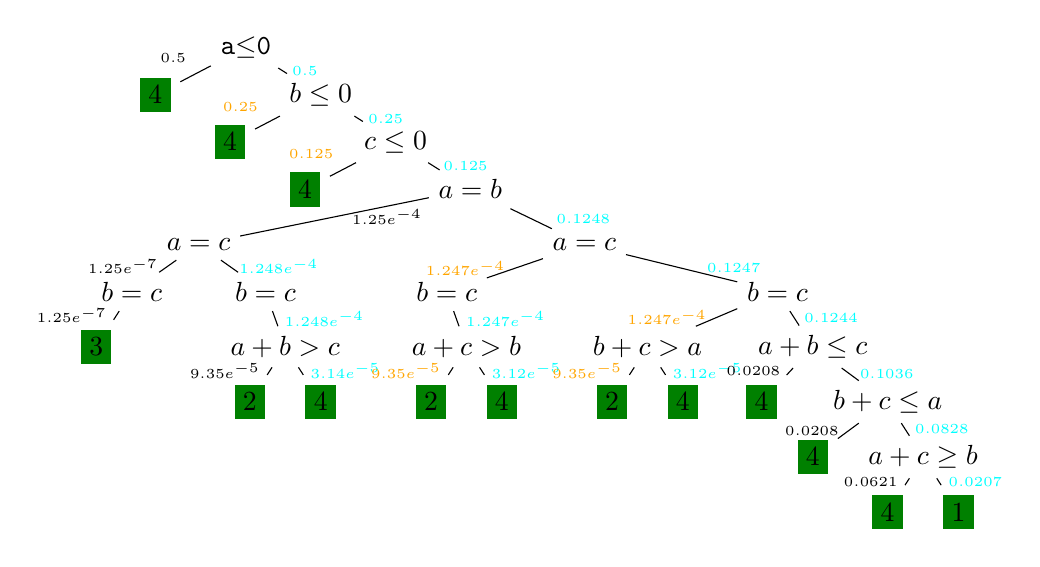
\begin{tikzpicture}[scale=0.6]
  \node {\texttt{a$\le$0}}
     child [color=black] {
       node[xshift=-7mm, yshift=3mm] {\colorbox{Green}{4}}
       edge from parent
       node[left, yshift=2mm] {\tiny $0.5$}
     }
     child [color=black] {
       node[xshift=5mm, yshift=3mm] {$b \le 0$}
       child {
         node[xshift=-7mm, yshift=3mm] {\colorbox{Green}{4}}
         edge from parent
         node[left, yshift=2mm] {\tiny \color{Orange}{$0.25$}}
       }
       child {
         node[xshift=5mm, yshift=3mm] {$c \le 0$}
         child {
           node[xshift=-7mm, yshift=3mm] {\colorbox{Green}{4}}
           edge from parent
           node[left, yshift=2mm] {\tiny \color{Orange}{$0.125$}}
         }
         child {
           node[xshift=5mm, yshift=3mm] {$a=b$}
           child {
             node[xshift=-30mm, yshift=2mm] {$a=c$}
             child {
               node[xshift=-4mm, yshift=3mm] {$b=c$}
               child {
                 node[xshift=0mm, yshift=2mm] {\colorbox{Green}{3}}
                 edge from parent
                 node[left] {\tiny $1.25e^{-7}$}
               }
               child [color=white] {
                 node[xshift=0mm, yshift=2mm] {\colorbox{white}{\textcolor{white}{3}}}
                 edge from parent
               }
               edge from parent
               node[left] {\tiny $1.25e^{-7}$}
             }
             child {
               node[xshift=4mm, yshift=3mm] {$b=c$}
               child [color=white] {
                 node[xshift=-2mm, yshift=2mm] {\colorbox{white}{\textcolor{white}{3}}}
                 edge from parent
               }
               child { 
                 node[xshift=-2mm, yshift=2mm] {$a+b>c$}
                 child {
                   node[yshift=2mm] {\colorbox{Green}{2}}
                   edge from parent
                   node[left] {\tiny $9.35e^{-5}$}
                 }
                 child {
                   node[yshift=2mm] {\colorbox{Green}{4}}
                   edge from parent
                   node[right] {\tiny \color{Cyan}{$3.14e^{-5}$}}
                 }
                 edge from parent
                 node[right] {\tiny \color{Cyan}{$1.248e^{-4}$}}
               }
               edge from parent
               node[right] {\tiny \color{Cyan}{$1.248e^{-4}$}}
             }
             edge from parent
             node[right, xshift=1mm] {\tiny {$1.25e^{-4}$}}
           }
           child {
             node[xshift=10mm, yshift=2mm] {$a=c$}
             child {
               node[xshift=-13mm, yshift=3mm] {$b=c$}
               child [color=white] {
                 node[xshift=-2mm, yshift=2mm] {\colorbox{white}{\textcolor{white}{3}}}
                 edge from parent
               }
               child {
                 node[xshift=-2mm, yshift=2mm] {$a+c>b$}
                 child {
                   node[yshift=2mm] {\colorbox{Green}{2}}
                   edge from parent
                   node[left] {\tiny \color{Orange}{$9.35e^{-5}$}}
                 }
                 child {
                   node[yshift=2mm] {\colorbox{Green}{4}}
                   edge from parent
                   node[right] {\tiny \color{Cyan}{$3.12e^{-5}$}}
                 }
                 edge from parent
                 node[right] {\tiny \color{Cyan}{$1.247e^{-4}$}}
               }
               edge from parent
               node[left] {\tiny \color{Orange}{$1.247e^{-4}$}}
             }
             child {
               node[xshift=20mm, yshift=3mm] {$b=c$}
               child {
                 node[xshift=-12mm, yshift=2mm] {$b+c>a$}
                 child {
                   node[yshift=2mm] {\colorbox{Green}{2}}
                   edge from parent
                   node[left] {\tiny \color{Orange}{$9.35e^{-5}$}}
                 }
                 child {
                   node[yshift=2mm] {\colorbox{Green}{4}}
                   edge from parent
                   node[right] {\tiny \color{Cyan}{$3.12e^{-5}$}}
                 }
                 edge from parent
               node[left] {\tiny \color{Orange}{$1.247e^{-4}$}}
               }
               child {
                 node[xshift=0mm, yshift=2mm] {$a+b \le c$}
                 child {
                   node[xshift=-2mm, yshift=2mm] {\colorbox{Green}{4}}
                   edge from parent
                   node[left] {\tiny $0.0208$}
                 }
                 child {
                   node[xshift=5mm, yshift=2mm] {$b+c \le a$}
                   child {
                     node[xshift=-5mm, yshift=2mm] {\colorbox{Green}{4}}
                     edge from parent
                     node[left] {\tiny $0.0208$}
                   }
                   child {
                     node[xshift=0mm, yshift=2mm] {$a+c \ge b$}
                     child {
                       node[yshift=2mm] {\colorbox{Green}{4}}
                       edge from parent
                       node[left] {\tiny $0.0621$}
                     }
                     child {
                       node[yshift=2mm] {\colorbox{Green}{1}}
                       edge from parent
                       node[right] {\tiny \color{Cyan}{$0.0207$}}
                     }
                     edge from parent
                     node[right] {\tiny \color{Cyan}{$0.0828$}}
                   }
                   edge from parent
                   node[right] {\tiny \color{Cyan}{$0.1036$}}
                 }
                 edge from parent
                 node[right] {\tiny \color{Cyan}{$0.1244$}}
               }
               edge from parent
               node[right,xshift=2mm] {\tiny \color{Cyan}{$0.1247$}}
             }
             edge from parent
             node[right,xshift=2mm] {\tiny \color{Cyan}{$0.1248$}}
           }
           edge from parent
           node[right] {\tiny \color{Cyan}{$0.125$}}
         }
         edge from parent
         node[right] {\tiny \color{Cyan}{$0.25$}}
       }
       edge from parent
       node[right] {\tiny \color{Cyan}{$0.5$}}
     };
\end{tikzpicture}
\end{center}
\end{frame}

\begin{frame}{Probabilistic symbolic execution tree}
\begin{center}
\pgfdeclarelayer{foreground}
\pgfsetlayers{main,foreground}
\begin{tikzpicture}[scale=0.6]
  \node {\texttt{a$\le$0}}
     child [color=black] {
       node[xshift=-7mm, yshift=3mm] {\colorbox{Green}{4}}
       edge from parent
       node[left, yshift=2mm] {\tiny $0.5$}
     }
     child [color=black] {
       node[xshift=5mm, yshift=3mm] {$b \le 0$}
       child {
         node[xshift=-7mm, yshift=3mm] {\colorbox{Green}{4}}
         edge from parent
         node[left, yshift=2mm] {\tiny \color{Orange}{$0.25$}}
       }
       child {
         node[xshift=5mm, yshift=3mm] {$c \le 0$}
         child {
           node[name=ref, xshift=-7mm, yshift=3mm] {\colorbox{Green}{4}}
           edge from parent
           node[left, yshift=2mm] {\tiny \color{Orange}{$0.125$}}
         }
         child [color=white] {
           node[xshift=5mm, yshift=3mm] {$a=b$}
           child {
             node[xshift=-30mm, yshift=2mm] {$a=c$}
             child {
               node[xshift=-4mm, yshift=3mm] {$b=c$}
               child {
                 node[xshift=0mm, yshift=2mm] {}
                 edge from parent
               }
               child [color=white] {
                 node[xshift=0mm, yshift=2mm] {}
                 edge from parent
               }
               edge from parent
             }
             child {
               node[xshift=4mm, yshift=3mm] {$b=c$}
               child [color=white] {
                 node[xshift=-2mm, yshift=2mm] {}
                 edge from parent
               }
               child { 
                 node[xshift=-2mm, yshift=2mm] {$a+b>c$}
                 child {
                   node[yshift=2mm] {}
                   edge from parent
                 }
                 child {
                   node[yshift=2mm] {}
                   edge from parent
                 }
                 edge from parent
               }
               edge from parent
             }
             edge from parent
           }
           child {
             node[xshift=10mm, yshift=2mm] {$a=c$}
             child {
               node[xshift=-13mm, yshift=3mm] {$b=c$}
               child [color=white] {
                 node[xshift=-2mm, yshift=2mm] {}
                 edge from parent
               }
               child {
                 node[xshift=-2mm, yshift=2mm] {$a+c>b$}
                 child {
                   node[yshift=2mm] {}
                   edge from parent
                 }
                 child {
                   node[yshift=2mm] {}
                   edge from parent
                 }
                 edge from parent
               }
               edge from parent
             }
             child {
               node[xshift=20mm, yshift=3mm] {$b=c$}
               child {
                 node[xshift=-12mm, yshift=2mm] {$b+c>a$}
                 child {
                   node[yshift=2mm] {}
                   edge from parent
                 }
                 child {
                   node[yshift=2mm] {}
                   edge from parent
                 }
                 edge from parent
               }
               child {
                 node[xshift=0mm, yshift=2mm] {$a+b \le c$}
                 child {
                   node[xshift=-2mm, yshift=2mm] {}
                   edge from parent
                 }
                 child {
                   node[xshift=5mm, yshift=2mm] {$b+c \le a$}
                   child {
                     node[xshift=-5mm, yshift=2mm] {}
                     edge from parent
                   }
                   child {
                     node[xshift=0mm, yshift=2mm] {$a+c \ge b$}
                     child {
                       node[yshift=2mm] {}
                       edge from parent
                     }
                     child {
                       node[yshift=2mm] {}
                       edge from parent
                     }
                     edge from parent
                   }
                   edge from parent
                 }
                 edge from parent
               }
               edge from parent
             }
             edge from parent
           }
           edge from parent
         }
         edge from parent
       }
       edge from parent
     };

   \begin{pgfonlayer}{foreground}
      \pause
      \node[name=first, yshift=5mm, xshift=30mm, below of=ref] 
         {$\x{slice}( true, a\le0) = true$};\pause
      \node[name=second, below of=first, yshift=5mm] 
         {$p_c = \x{prob}(a \le 0)/\x{prob}(true)$};\pause
      \node[name=third, below of=second] 
         {$\x{slice}( a\le0 \wedge b\le0, c\le0) = true$};\pause
      \node[name=fourth, below of=third, yshift=5mm] 
         {$p_c = \x{prob}(c \le 0)/\x{prob}(true)$};\pause
      \node[name=fourth, below of=fourth] 
         {Normalization of constraints, e.g., $a \mapsto v_1$, $c \mapsto v_1$, enables reuse in calculating $p_c$};
   \end{pgfonlayer}

\end{tikzpicture}
\end{center}
\end{frame}

\begin{frame}{Calculating $\x{prob}(\cdot)$}
We report on support for linear integer arithmetic (LIA) constraints
using LattE
\begin{itemize}
\item computes the number of {\em lattice} points in 
a convex polytope;
\item constraints encoded as system of inequalities, $A x \le B$; 
\item does not support disjunction or disequality constraints, i.e., $x \not= c$
\end{itemize}
\pause
Our calculation relies on ``counting'' the number of solutions of a set
of related constraints using LattE and combining the results.
\begin{itemize}
\item $\x{count} = \x{count}_{\wedge}(\bigwedge_{\x{ineqSet}}) - \x{count}_{\vee}(\bigvee_{\x{exSet}})$
\item \texttt{return} $\x{count} / \prod_{v \in \x{vars}} \x{dom}(v)$
\end{itemize}
\end{frame}

\begin{frame}{$\alpha \wedge (x \not= 0) \wedge (y \not=0)$ cannot be expressed directly}
\begin{center}

\def\firstcircle{(0,0) circle (1.5cm)}
\def\secondcircle{(45:2cm) circle (1.5cm)}
\def\thirdcircle{(0:2cm) circle (1.5cm)}

\begin{tikzpicture}[scale=1.0]
\pause
    \draw \firstcircle node[below] {$\alpha$};
    \node[yshift=-30mm] {Count the solutions to $\alpha$};

\end{tikzpicture}
\end{center}
\end{frame}

\begin{frame}{$\alpha \wedge (x \not= 0) \wedge (y \not=0)$ cannot be expressed directly}
\begin{center}

\def\firstcircle{(0,0) circle (1.5cm)}
\def\secondcircle{(45:2cm) circle (1.5cm)}
\def\thirdcircle{(0:2cm) circle (1.5cm)}

\begin{tikzpicture}[scale=1.0]
    \draw \firstcircle node[below] {$\alpha$};
    \draw \secondcircle node [above] {$x=0$};

    \begin{scope}
      \clip \firstcircle;
      \fill[red] \secondcircle;
    \end{scope}
    \node[yshift=-30mm] {Remove the count of solutions to $\alpha \wedge (x=0)$};

\end{tikzpicture}
\end{center}
\end{frame}

\begin{frame}{$\alpha \wedge (x \not= 0) \wedge (y \not=0)$ cannot be expressed directly}
\begin{center}
\def\firstcircle{(0,0) circle (1.5cm)}
\def\secondcircle{(45:2cm) circle (1.5cm)}
\def\thirdcircle{(0:2cm) circle (1.5cm)}

\begin{tikzpicture}[scale=1.0]
    \draw \firstcircle node[below] {$\alpha$};
    \draw \thirdcircle node [below] {$y=0$};

    \begin{scope}
      \clip \firstcircle;
      \fill[blue] \thirdcircle;
    \end{scope}
    \node[yshift=-30mm] {Remove the count of solutions to $\alpha \wedge (y=0)$};

\end{tikzpicture}
\end{center}
\end{frame}


\begin{frame}{$\alpha \wedge (x \not= 0) \wedge (y \not=0)$ cannot be expressed directly}
\begin{center}
\def\firstcircle{(0,0) circle (1.5cm)}
\def\secondcircle{(45:2cm) circle (1.5cm)}
\def\thirdcircle{(0:2cm) circle (1.5cm)}

\begin{tikzpicture}[scale=1.0]
    \draw \firstcircle node[below] {$\alpha$};
    \draw \secondcircle node [above] {$x=0$};
    \draw \thirdcircle node [below] {$y=0$};

    \begin{scope}
      \clip \firstcircle;
      \clip \secondcircle;
      \fill[green] \thirdcircle;
    \end{scope}
    \node[yshift=-30mm] {Add back the count of solutions to $\alpha \wedge (x=0) \wedge (y=0)$};

\end{tikzpicture}
\end{center}
\end{frame}

\begin{frame}{$\alpha \wedge (x \not= 0) \wedge (y \not=0)$ cannot be expressed directly}
\begin{center}
\def\firstcircle{(0,0) circle (1.5cm)}
\def\secondcircle{(45:2cm) circle (1.5cm)}
\def\thirdcircle{(0:2cm) circle (1.5cm)}

\begin{tikzpicture}[scale=1.0]
    \begin{scope}
        \begin{scope}[even odd rule]% first circle without the second
            \clip \secondcircle (-3,-3) rectangle (3,3);
            \clip \thirdcircle (-3,-3) rectangle (3,3);
        \fill[yellow] \firstcircle;
        \end{scope}
        \draw \firstcircle node {$\alpha$};
        \draw \secondcircle node {$x=0$};
        \draw \thirdcircle node {$y=0$};
    \end{scope}
       \node[name=ref, below, yshift=-20mm] {This results in the count of $\alpha \wedge (x\not=0) \wedge (y\not=0)$};
\pause
       \node[below of=ref, yshift=5mm] {Complexity is exponential in number of disequality constraints};
    
\end{tikzpicture}
\end{center}
\end{frame}

\begin{frame}{Optimizing $\x{count}_{\wedge}(\cdot)$}
Our experience with LattE revealed that its execution time
\begin{itemize}
\item is not dependent on the size of variable domains;
\item is highly dependent on the number of variables (dimension of the polytope);
\item is highly dependent on the number of constraints (faces of the polytope);
\end{itemize}
\pause
Our experience with sliced PCs revealed that
\begin{itemize}
\item a significant portion of the PC, and many variables, can be eliminated;
\item sliced PCs, if normalized, recur throughout the symbolic execution tree
\end{itemize}
\pause
Our implementation of $\x{count}_{\wedge}(\cdot)$ 
\begin{itemize}
\item normalizes the inequality system
\item caches the counts computed for each system; and 
\item checks the cache before invoking LattE.
\end{itemize}
\end{frame}

\begin{frame}{How well does this work?}
Our ISSTA 2012 paper describes several usage scenarios ...
\begin{itemize}
\item finding a bug by looking at anomalies in path probabilities;
\item assessing the probability of covering lines of code; and
\item characterizing the likelihood of detected bugs
\end{itemize}
\vfill
\pause
I'll focus on the necessity of the optimizations we've developed.
\end{frame}

\begin{frame}{Memoization and Slicing are key}
\begin{center}
\begin{itemize}
\item Ran on Binomial Heap and TreeMap collections with all possible input sequences (adds, removes, etc.) of length 4;
\item times reported in seconds\pause
\end{itemize}
\vfill
{\footnotesize
\begin{tabular}{cccccccccc}
\hline
Subject  & Memoize & Slice & PC & Var & $\x{prob}(\cdot)$ & LattE & Reused & LattE & Total \\ 
& & & Red. & Red.  & & & & time & time \\ \hline
Binomial & \ON         & \ON     & $55\%$ & $67\%$   & $634$ & $~~518$ & $~370$   & $~~35$ & $~~57$ \\         & \OF         & \ON     & $55\%$ & $67\%$   & $634$ & $~~888$ & $~~~0$ 
  & $~~61$ & $~~84$ \\
         & \ON         & \OF     & $~0\%$ & $~0\%$   & $634$ & $~3160$ & $~698$   & $~388$ & $~414$ \medskip\\TreeMap  & \ON         & \ON     & $44\%$ & $55\%$   & $766$ & $~2264$ & $~562$   & $~118$ & $~145$ \\         & \OF         & \ON     & $44\%$ & $55\%$   & $766$ & $~2826$ & $~~~0$   & $~150$ & $~178$ \\
         & \ON         & \OF     & $~0\%$ & $~0\%$   & $766$ & $12108$ & $4965$   & $1028$ & $1056$ \\
\hline
\end{tabular}
}
\end{center}
\end{frame}

\begin{frame}{Availability and Ongoing work}
An SPF extension that implements our approach is available
\begin{itemize}
\item \url{http://probsym.googlecode.com}
\item improved over results in paper; uses our new solver interface
{\color{Green}{Green}}
\item \url{http://green-solver.googlecode.com}
\end{itemize}
\pause
We have added or are working on ...
\begin{itemize}
\item support for structures, scheduling and other ``choice''s in JPF;
\item confidence-based samplers when model counting is not available; 
\item support for user defined input probability distributions; and
\item additional constraint theories
\end{itemize}
\end{frame}

\begin{frame}{Future of SE}
There are numerous high-impact opportunities 
\begin{itemize}
\item exploiting emerging technologies
\item targetting domain-specific development challenges
\end{itemize}
\vfill
To leverage those opportunities
\begin{itemize}
\item you need to invest time/effort
\item it is extremely helpful to have a willing partner
\end{itemize}
\end{frame}

\begin{frame}
	\titlepage %displays the title page
\end{frame}

\end{document}
